\chapter[PHARMACOKINETICS]{\textbf{DRUG CONCENTRATION WITHIN THE FIELD OF PHARMACOKINETICS}}
\thispagestyle{empty}
\numberwithin{equation}{chapter}


\section{DRUG CONCENTRATION IN SINGLE COMPARTMENT SYSTEM}
\par ~~~~~~~~~~Mathematical model in pharmacokinetics often describe the evolution of pharmacological process in terms of system of linear or non-linear ordinary differential equations. It helps us to decide the step suitable for maintain constant drug level in the body of a patient. It shows that under certain condition these are limiting values for measurement minimum concentration of the drug and amount of drug at a given time in the body of a patient.

\par ~~~~~~~~~~We need to find time interval between application be chosen so that the concentration doesn't become so large as to be dangerous as small as to be ineffective. The objective of the work is to show how one can read this ODE's and draw conclusion from them about the qualitative behaviour of the pharmacological processes that is being modelled. The model could improve human health from helping a doctor to optimize patient doses to stream lining the early stages of pharmaceutical research.

\section*{HISTORY}
~~~~~~~~~~~~There is a killer found in many household medicine cabinets  Tylenol which was marketed as a pain reliever in 1950. US CDC estimated there were 1,600 deaths from Tylenol poisoning between 2001 and 2010 which is the most common cause of acute hepatic failure and was the second most common cause of liver failure. The United States government’s Food and Drug Administration (FDA) provides recommendations for dosages and frequency of use.
This is a classic problem in pharmacokinetics using first-order differential equation. The field of pharmacokinetics and the related field of pharmacodynamics are mature and sophisticated fields that use mathematics to merge physiology, pharmacology, and medicine for planning safe drug usage.
 

\subsection{Drug Dose Providing Periodically}

\par ~~~~~~~~Let $y=y(t)$ be the quality of the drug concentration in the patient’s body at time t. Initially at time t=0 say patients given a dose, say $y_{0}$ of the drug.
\par ~~~~~~~~~~~~As a first approximation we let drug disappears from the body according to the law $\frac{dy}{dt}=-ky$ \\
The value of the constant k depending on the particular drug used.\\
$\frac{dy}{dt}+ky=0$ $\Rightarrow$ $y=y_{0}e^{-kt}$ \\
After a set interval T say an equal
amount of the drug $y_{0}$ added so that the concentration at time T is 
$$y(T)=y_{0}+e^{-kT}$$
Similarly as $t\rightarrow 2T$ the concentration will approach $(y_{0}+y_{0}e^{-kT})e^{-kT}$ and after adding another dose $y_{0}$ the concentration at time 2T is 
$$y(2T)=y_{0}+(y_{0}+y_{0}e^{-kT})e^{-kT}=$$ 
$$~~~~~~~~~=y_{0}(1+e^{-kT}+e^{-2kT})e^{-2kT}$$ 
In the same way after another dose at time 3T, the concentration is given by 
$$y(3T)=y_{0}(1+e^{-kT}+e^{-2kT}+e^{-3kT})$$ 
and continuing in this way at time nT
$$y(nT)=y_{0}(1+e^{-kT}+e^{-2kT}+...e^{-nkT})$$
This is a geometric progression and can be summed to give
$$y(nT)=y_{0}(\frac{e^{-nkT}-1}{e^{-kT}-1})$$
For large n $~~~~~~~~~~~~~~~~~~~~~~y\rightarrow \frac{y_{0}}{1-e^{-kT}}$ \\
So the if the dosage level is required to approach the level $y_{c}$, we must have $y_{c}=\frac{y_{0}}{1-e^{-kT}}$ \\
Hence for a given time interval T, the required dosage is given.
\par ~~~~~~~~Clearly one of the advantage of this accumulation is its slowness in approaching the limiting value y. So that at the end of first interval T, the concentration is given by $y_{c}e^{-kT}$.\\ We now add a dose say $y_{1}$ which returns the level to $y_{c}$ \\
ie,  \begin{center}
	$$y_{1}+y_{c}e^{-kT}=y_{0}$$
	$\Rightarrow$  $y_{1}=y_{c}(1-e^{-kT})=y_{0}$
\end{center}
Thus we continue giving doses yo at time intervals T after the initial dose $y_{c}$. This second method has the advantage of bringing the body concentration straight to the required level, but this can also be disadvantage as a large initial dose can have side effects on the body.
%(graph)
%GRAPH

\begin{center} %Align the Image
		\scalebox{0.80} % Scale down to 70 /% of the original size!
		{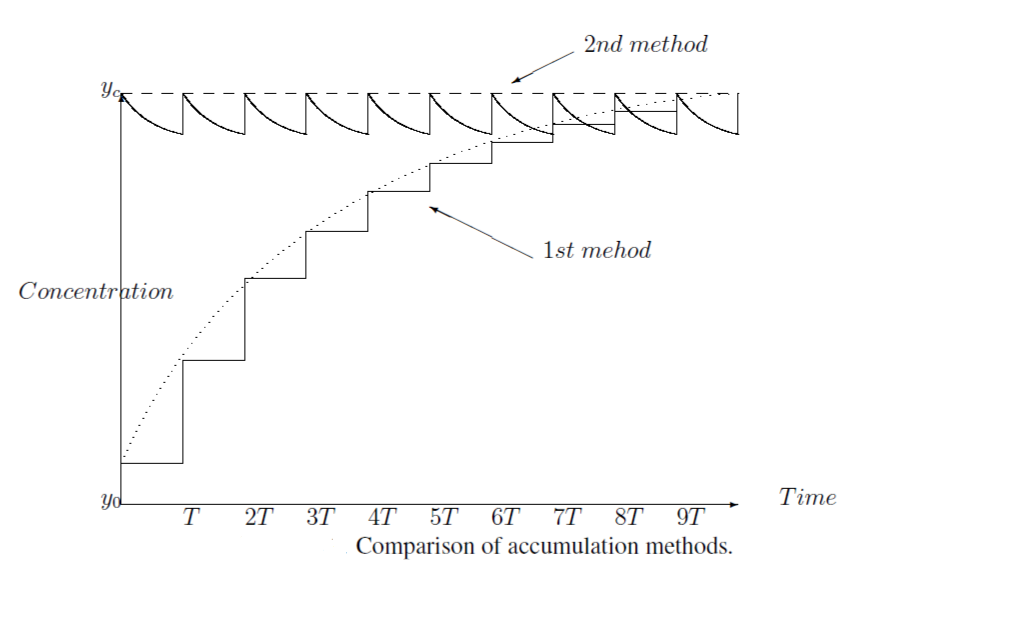
\includegraphics{graph7.png}} 
\end{center}


\subsection{Drug Dose Providing at Regular Interval}
\par ~~~~~~~~~~Now consider the case of patient is given a dose yo of drug at regular intervals of time T. The body concentration of the approximately obeys the law
$$\frac{dy}{dt}=-ke^{y}$$
$~~~~~~~~~~~~~~~~~~~~~~~~~~~~~~~~~~\Rightarrow$  $y=-\log (kT+c)$ \\
The concentration $y_{1}$, just before the second dose
$$y_{1}=-log(kT+e^{-y_{0}})$$
And the concentration $y_{2}$ just before the third dose is 
$$y_{2}=-log(kT+e^{-(y_{0}+y_{1})})$$

Consider,$$e^{-(y_{0}+y_{1})}=e^{-y_{0}}(kT+e^{-y_{0}})$$
$$y_{2}=-log(kT+e^{-y_{0}}(kT+e^{-y_{0}}))$$
$$~~=-\log (kT(1+e^{-y_{0}})+e^{-2y_{0}})$$
Similarly $$y_{3}=-\log (kT+e^{-(y_{0}+y_{2})})$$

Consider $$e^{-(y_{0}+y_{2})}=kT(e^{-y_{0}}+e^{-2y_{0}})+e^{-3y_{0}}$$
$~~~~~~~~~~~~~~~~~~~~~~\Rightarrow$  $~~~~~~~~y_{3}=-\log(kT(1+e^{-y_{0}}+e^{-2y_{0}})+e^{-3y_{0}})$ \\

Proceeding like this, we get,
$$~~~~~~~~~~~~y_{n}=-\log(kT(1+e^{-y_{0}}+e^{-2y_{0}}...+e^{-(n-1)y_{0}})+e^{-ny_{0}})$$
$$=-\log(kT[\frac{1-e^{-ny_{0}}}{1-e^{-y_{0}}}+e^{-ny_{0}}])~~~~~~~~~~$$
For n tends to c $(y_{n}\rightarrow y_{c})$ the doses becomes larger and
$$y_{c}=-\log\frac{kT}{1-e^{-y_{c}}}$$
\begin{center}
	$\Rightarrow$ $T=\frac{e^{-y_{c}}}{k}(1-e^{-y_{c}})$
\end{center} 
This is time required to alter the certain concentration $y_{c}$ from the first dose. 





\pagebreak


\section{CONCENTRATION OF A DRUG IN A TWO COMPARTMENT SYSTEM}


\par ~~~~~~~~~~~~Compartmental models have proven extremely useful in predicting drug concentration levels in organs and in estimating rates at which a drug is eliminated from the body. A simple two compartment model for describing the kinetics of a metabolic process is the situation in which the drug is passes through two separate locations within the body including blood, organs, tissues and urine. This effect the amount of the drug in the body because now it is being metabolized in two places at different rates.

\subsection*{Mathematical Model}

%GRAPH
\begin{center}
	
	\scalebox{0.70} % Scale down to 70 /% of the original size!
	{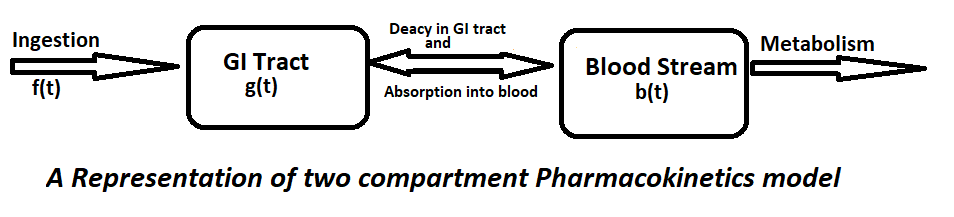
\includegraphics{graph8.png}}
\end{center}

\par ~~~~~~~~~~We shall determine here the concentration of some chemicals, such as a drug, in a system consisting of two compartments separated by a membrane. The drug can pass through this membrane from compartment I to Compartment 2, or vice versa. We also assume that the drug can escape to the external system through an opening in the second compartment.


\par ~~~~~~~~~~Let $V_{1}$ and $V_{2}$ be the volumes of the two compartments and A is the cross sectional area of the membrane.  Also, let g(t) and b(t) denote the masses of the drug in compartments 1 and 2 respectively. 
Let Gastrointestinal tract(GI) and blood stream are the two compartments.\\

~~~~~~~~~~~~~~~~~~~~~~Rate of change of drug mass in GI$= \frac{dg(t)}{dt}$ \\
Rate of flow of drug mass from blood stream to GI$= a_{2_{1}}\frac{Ab(t)}{V_{2}}$ \\


(Since the rate of flow of the drug from GI to blood is proportional to area A of membrane and concentration of drug in blood=$ \frac{b(t)}{V_{2}}$)where $a_{2_{1}}$ is the constant of proportionality.
\par ~~~~~~~~~~~~~~~~~~Similarly Rate of flow of drug from GI to blood $=a_{1_{2}} \frac{Ag(t)}{V_{1}}$ \\ where $a_{1_{2}}$ is the constant of proportionality. 
\linebreak
\\
\begin{flushright}
	Now~~~~~~~~~~~~, Rate of change of drug in GI tract = Rate of flow of drug from\\ blood to GI tract -Rate of flow of drug from GI to blood stream.\\
\end{flushright}
ie, \begin{equation*}
\frac{dg(t)}{dt}=a_{2_{1}}\frac{Ab(t)}{V_{2}}-a_{1_{2}}\frac{Ag(t)}{V_{1}}
\end{equation*}
\\
Similarly corresponding equation for blood stream yields, 
\begin{flushright}
	Rate of change of drug mass in blood stream= Rate of flow of drug from\\ GI to blood - Rate of flow of drug from blood to GI -\\ Rate of flow of drug from blood into the external system.
\end{flushright}
\begin{equation*}
\frac{db(t)}{dt}=a_{1_{2}}\frac{Ag(t)}{V_{1}}-a_{2_{1}}\frac{Ab(t)}{V_{2}}-a\frac{b(t)}{V_{2}}
\end{equation*}
Now substituting   $$\beta=a_{2_{1}}\frac{A}{V_{2}}$$
$$\alpha=a_{1_{2}}\frac{A}{V_{1}}$$
$$f(t)=\frac{a}{V_{2}}$$

Hence above equation take the form
$$\frac{dg(t)}{dt}=f(t)-\beta g(t)$$
$$\frac{db(t)}{dt}=\beta g(t)-\alpha b(t)$$

In this instance,
\\b(t)=amount of drug in the blood stream at time t
\\g(t)=amount of drug in GI tract
\\$\alpha =$ metabolism of drug in the blood stream
\\$\beta =$  metabolism of drug in the GI tract

\par This is a non homogeneous equation because f(t) doesn't play a direct role on the other functions. So to solve we want to turn the system into a second order linear equation.
$$~~~~~~~~~~[\frac{d}{dt}+\beta][g(t)]=0$$
$$[\frac{d}{dt}+\alpha][b(t)]-\beta g(t)=0$$
or 
$$~~~~~~~~~~[D+\beta][g(t)]=0$$
$$[D+\alpha]\beta(t)-\beta g(t)=0$$
where D represents derivative in terms of t and f(t)=1

\par We want g(t) terms to have the same coefficient, solve by elimination. So we multiply the top equation by $\beta$ and bottom equation bt $D+\beta$
\\Hence $$ ~~~~~~~~~~~~~~~~\beta[D+\beta]g(t)=0$$
$$[D+\alpha][D+\beta]b(t)-\beta [D+\beta]g(t)=0~~~~~~~$$
Adding we get $$~~~~~~~~~~~~~~[D+\alpha][D+\beta][b(t)]=0$$
$$ \Rightarrow  ~~~~~~~~[D^{2}+(\alpha +\beta)D+\alpha \beta]b(t)=0~~~~$$

This is a second order linear equation.~\\
 $$Here~~~~~~~~~[D+\beta][D+\alpha]=0~~~~$$
$$~~~\Rightarrow~~~~~~~~~~~~~~~~~~~~~ D=-\beta$$  $$~~~~or~~~~~~~~~~~~~~~~~~~~~~~~D=-\alpha$$

There for homogeneous solution is $b_{h}=Ae^{-\alpha t}+Be^{-\beta t}$ \\
We must consider the particular solution since the system is non-homogenous.
\par Here the particular solution is $b_{p}=\frac{1}{\alpha}$\\
So our complete equation is $$b(t)=Ae^{-\alpha t}+Be^{-\beta t}+\frac{1}{\alpha}$$
Here b(t) is the amount of drugs in the bloodstream in terms of time t, A and B are drug amount of two compartments and $\alpha$ and $\beta$ are decay rate constants for each compartment.
\par Using this model we can determine the amount of drug in the blood at any given time when the drug passes through two compartments.

\subsection*{Example}
\textit{{\Large Lidocain Metabolism:}} The drug Lidocain is commonly used in the treatment of irregular heartbeat. We assume that 2mg of Lidocain are injected into the bloodstream and then move into the heart tissues.
\\Hence \begin{center}
	
	$\frac{dg}{dt}=-g(t)+2~~~~~~~~~~~~~~~~~~$ ,     
	g(0)=0  \\
	$\frac{db}{dt}=-g(t)-b(t)~~~~~~~~~~~~~~~~~~$        ,      b(0)=0
\end{center} 
Gives
\begin{center}
	$g(t)=2e^{-t}$ \\
	$b(t)=2e^{-t}$
\end{center}
The schematic model shown in the figure below is widely used model of lidocaine kinetics.

%GRAPH

\begin{center} %Align the Image
	\scalebox{1.20} % Scale down to 70 /% of the original size!
	{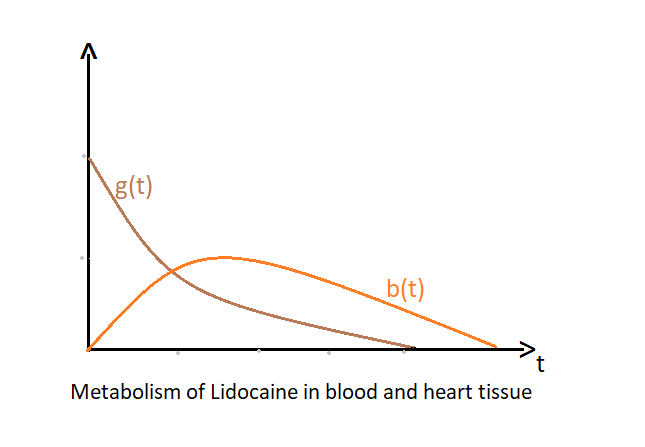
\includegraphics{graph8(2).png}} %include the image - image is in the working folder
	%\caption{} \label{altbin1} %Caption of the image and label
\end{center}




\pagebreak



\section{ABSORPTION OF DRUGS IN ORGANS OR CELLS}



\par ~~~~~~~~~~For purposes of mathematical analysis in biology, it is often convenient to consider an organism (such as a human, animal or plant) as a collection of individual components called "compartments". A compartment may be an organ (such as the stomach, pancreas or liver) or a group of cells which together act as a unit. 

\par ~~~~~~~~~~~~An important problem consists in determining the absorption of chemicals, such as drugs by cells or organs. This has practical applications in the field of medicine and the simplest type of problem deals only with one compartment.

\par ~~~~~~~~~~The following example will serve to illustrate the kind of problems which can arise.

\subsection*{Example}
~~~~~~~~~~~~A liquid carries a drug into an organ of volume $V cm^{3}$ at a rate $\alpha cm^{3}/s$ and leaves at a rate $\beta cm^{3}/s$. The concentration of the drug in entering liquid  is $c g/cm^{3}$. \\ (a) Write a differential equation for the concentration of the drug in the  organ at any time together with suitable conditions \\
(b) solve the equation. ~\\

\textit{\Large Solution}\\

\par ~~Figure shows a single compartment of volume V together  with an inlet and an outlet. Let x be the concentration of drugs in the organ, then  the amount of the drug in the organ at any time t is      
$(V cm^{3})(x g/cm^{3}) = xV g$ .\\

%figure

\begin{center} %Align the Image
	\scalebox{1.00} % Scale down to 70 /% of the original size!
	{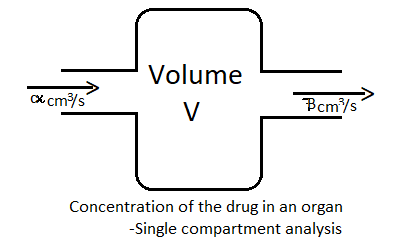
\includegraphics{graph9.png}} %include the image - image is in the working folder
	%\caption{} \label{altbin1} %Caption of the image and label
\end{center}


The amount entering the organ at any time t is
$$(\alpha cm^{3}/s) (c g/cm^{3}) = \alpha c  g/s $$	
and the amount leaving the organ is
$$(\beta cm^{3}/s) (x g/cm^{3}) = \beta x g/s $$

Now, the differential equation describing the present situation is given by 
$$\frac{d}{dt}(xV)= \alpha c– \beta x $$ 
and the suitable conditions are $x=x_{0}$ at $t=0$ \\
\linebreak 
(b) 
\begin{center}
	$~~~~~~~~~~~~~~~~~~\frac{dx}{dt}(xV)=\alpha c-\beta x$ \\
	$\Rightarrow~~~~~~~~~~$ 
	$~~~~~~~~~~~~V\dfrac{dx}{dt}=\alpha c-\beta x~~~~~~$ 
\end{center} 
Separating the variables we get solution of this equation as 
$$x=\frac{\alpha c}{\beta}+[x_{0}-\frac{\alpha c}{\beta}]e^{\frac{-\beta t}{V}}$$

We now have
\begin{itemize}
	
	\item \textit{Case I} \\
	When a=b. Here the rate at which the drug enters is same as the rate  at which the drug leaves 
	$$x=c+[x_{0}-c]e^{\frac{-\beta t}{V}}$$
	\item \textit{Case II} \\
	When a=b and $x_{0}=0$. That is, the inflow and outflow rates are equal  and the initial concentration of the drug in the organ is zero.
	$$x=c(1-e^{\frac{-\beta t}{V}})$$ 
\end{itemize}


